\chapter{Background}\section{Overview about image processing}
Nowadays, we have a lot of programs what used to edit the photos (e.g. photoshop, gimp, paint,...). By apply some technique, we can effectively some property to change the image such as: scaling, blurring, rotating image,.... Actually, an image is presented of a set of pixels. Each pixel carry a value which presented for the color at this location. When combine the value of all pixels, we have the image as we can see in the real word. The changing on image really changing the value on each pixel in image. Behind the techniques in these programs are mathematical operations and the field using mathematical operation on an input image,  called \textit{image processing}. The output of image processing may be either an image or a set of characteristics related to the image. And most of image processing technique are performed on two-dimensional image. In image processing, we have a lot of operations. In this chapter, we just introduce some basis operations what often useful for the object of this internship.
\section{Image filtering}
Image filtering is a process to modify or enhance the quality of images. This is known as a ``neighborhood" operation. The neighborhood is a set of pixels around a selected pixel. In image processing, with a pixel, we can have 4-neighbors or 8-neighbors of it. Image filtering determines the value at the selected pixel by apply some operations with the value of its neighbors. One of the filter operators is smoothing, also called blurring. This technique is used in preprocessing steps, particularly using for noise reduction. With a matrix called kernel. It was sliding over the image. At each position, the output of value at this position is average of its neighborhoods.
In image processing, we have many filter techniques. But it can be divided into 2 main types:\\[0.2cm]
\textbf{Linear filter}: The idea behind this filter is replacing the value of every pixel in the image by the average of the gray levels in the neighborhood defined by the filter mask. By this work, this filter sometime are called averaging filter. The result of this process is an image with reduced the sharp edges in gray level, it also reduce the noise because the noise is typically and random in the image. The mask is a matrix useful for blurring, sharpening, or edge-detection, .... The output image is accomplished by convoluting between a mask and an image.\\[0.2cm]
\textbf{Order-Statistics filter}: By ordering the pixels in the image and then replacing the value of the center pixel with the value determined by the ranking result. Median filter is an example of this technique.
\section{Histogram}
Histogram is a representation about distribution of data on the regions (we called bin) in the data range. The bins are the number of sub-ranges when we divide the entire data range into several small interval (i.e. With the range from 0 - 255 and the size of each sub-range (bin) is 16, the number of bins is $256/16 = 16$ bins. The first bin range is 0 - 15, the second range is 15 - 30, and so on). The value at each bin is the number of data which have value belong to this bin. Normally, histogram represented by the columns chart with x-axis represented for the number of bins, and y-axis represented for the value of each bin.\\
Histogram can be used effectively for image enhancement, also useful in many image processing applications, such as image compression and segmentation.\\[0.3cm]
\begin{figure}[h!]
\centering
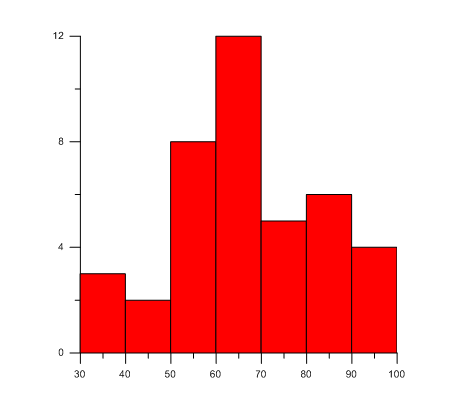
\includegraphics[scale=2]{images/histogram}
\caption{An example about histogram}
\label{fig:figure_31}
\end{figure}
\textbf{Histogram equation}: is a method allow adjust the contrast using the histogram of image. It mapping one distribution on a histogram to a wider distribution of intensity values. By this, the image can brighter.\\[0.2cm]
\textbf{Histogram matching}: is a method adjustment of two image using the histogram. This method was finished by calculating the cumulative distribution functions of two histograms and find the histogram matching function. Finally, apply the matching function on each pixel of the image to get the result.
\section{Segmentation}
Segmentation subdivides an image into its regions. The size of regions is depend on the problem being solved. This mean, segmentation should stop when the regions of interest in application have been detected. In the real, the segmentation was applied into many fields such as machine vision, medical imaging, object detection, etc. The most of segmentation algorithms are based on the basic properties of intensity values: discontinuity and similarity. In the first case, the segmentation based on abrupt changes in intensity. The second case, the image segmentation based on a predefined criteria. It means the image was segmented into regions that are similar according to a set of criteria. And, we have many the method to segment an image such as thresholding method, region growing, clustering method, histogram-based method, etc.\\[0.2 cm]
\textbf{Thresholding} is a simplest method of image segmentation. Thresholding use a particular threshold value ``t", we split the image into two parts: the first part includes pixels which have the value greater than t, and the second part contains the pixels vice versa. With this technique, thresholding can be used to create an binary image from a gray scale image. In fact, we have many type of threshold, as follows:
\begin{itemize}
\item \textit{Global thresholding}, when t is a constant over an entire image
\item \textit{Variable thresholding}, when t changes over an image
\item \textit{Local or regional thresholding}, is variable threshoding in a region of an image
\item \textit{Dynamic or adaptive thresholding}, if t depends on the spatial coordinates.
\item \textit{Multiple thresholding}, thresholding on 3 dominant modes (color image)
\end{itemize}
\textbf{Canny} algorithm is an edge detection algorithm that uses to detect the structure of image. The process of this algorithm can break into the steps follows \footnote{https://en.wikipedia.org/wiki/Canny\_edge\_detector}:
\begin{itemize}
\item Apply the Gaussian filter to smooth the image (remove the noise)
\item Find the intensity gradients of the image
\item Apply non-maximum suppression to get rid of spurious response to edge detection
\item Apply double threshold to determine potential edges
\item Track edges
\end{itemize}
\section{Color processing$^{\cite{oscarbook}}$}\label{color_model}
The use of color in image processing do not just identify or extract an objects from scene, it also a factor for image analysis. Color processing can be effect on each component image individually or work directly with pixels based on a color model. The color models is a specification of colors in some standard, generally accept way such as BGR, CMY, HSV or Grayscale model.
\begin{itemize}
\item BGR model: using blue, green, red as three primary colors. Image presented in this model consist of three components images for each primary color.
\item CMY model: used for hardcopy devices. Based on the BGR mode, each value in CMY mode was computed by integrate between 2 primary color in BGR. Specific, C (cyan) is consist from green and blue, M (magenta) is consist from red and blue and Y (yellow) is consist from red and green.
\item HSV model: difference with BGR, HSV using the 3 components are hue, saturation and brightness to present image. Hue is a color attribute which describe a pure color (yellow, orange, red) and saturation give a degree to pick the pure color is diluted by white light. Brightness is a notation of intensity for color sensation.
\item Grayscale model: The colors in grayscale just black and white because it just carry the intensity information on each pixel. Because that, the image in grayscale mode was called black and white image. The color of each pixels in image from black, where have weakest intensity to white at the strongest intensity.
\end{itemize}
The most color operations in image processing is transformation. This is a process to the conversion image between the color models by using a transform expression such as BGR to HSV, HSV to BGR, BGR to Grayscale.\\[0.2cm]
Besides that, considering the specific characteristic of each color space, allowing we can classify the pixels in the image. This idea can be used to segment object of an image. HSV model is widely used to compare the color because the range of color (Hue value) is specific.
\begin{figure}[h!]
\centering
\subfloat[An image in BGR mode]{\label{fig:example_1}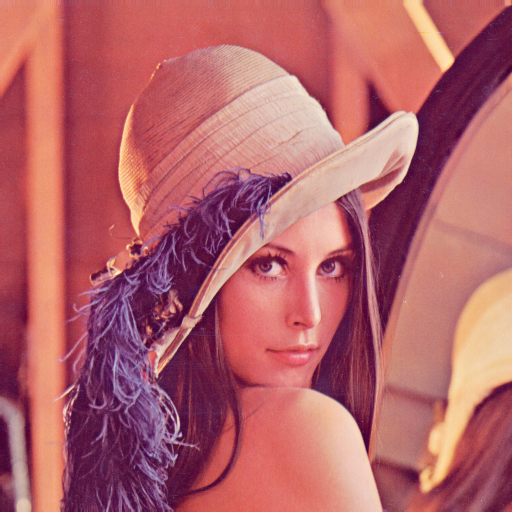
\includegraphics[width=0.4\textwidth]{./images/lenna}}~~
\subfloat[An image in Gray mode]{\label{fig:example_2}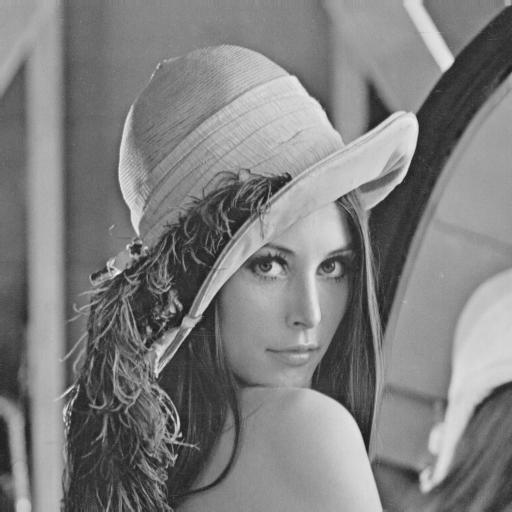
\includegraphics[width=0.4\textwidth]{./images/lenna_gray}}
\caption{The images with color transformation from BGR to Gray}
\label{fig:figure_31}
\end{figure}

